%\documentclass{article}
\documentclass[10pt,a4paper]{article}
\usepackage{fancyhdr}
\usepackage[margin=2.5cm]{geometry}
	\pagestyle{fancyplain}
% header on first page
		\fancyhf{}
			\lhead{\fancyplain{Proceedings}}
			\chead{}
			\rhead{\fancyplain{ECEM 2013}}
			\fancyfoot{} %please leave the footer blank
\renewcommand{\headrulewidth}{0pt}
\usepackage{color}
\usepackage{subfigure}
\usepackage{graphicx}
\usepackage{mathptmx}
\usepackage{multirow}
\usepackage[english]{babel}
\linespread{0.95}

\title{Interacting with Objects in the Environment by Gaze and Hand Gestures} %Fill this in

\date{} %keep date blank
\author{Jeremy Hales(jeremy.hales1@gmail.com)$^1$, Diako Mardanbeigi$^2$, David Rozado$^3$ \\ \\ %Fill in information
% for all authors here. Don't forget to include the email adress for the first author
$^1$University of Queensland - Department of Mechatronics \\ 
$^2$IT University of Copenhagen\\
$^3$ICT Centre - CSIRO} %Fill in affiliation information for all authors here. 


\begin{document}
\maketitle%\begin{center}

% \end{center} ---------------------------------------------------------------
\textbf{
\begin{center}
Abstract 
\end{center}
}%the initial 200 words from the submission page should be copied and pasted here
%---------------------------------------------------------------
\noindent
Head-mounted eye trackers can be used for mobile gaze estimation. In this paper we use low-cost hardware to build a
set of gaze tracking glasses and an open-source based gaze estimation algorithm that in combination with a video-based
hand gesture recognition algorithm allows the user of the glasses to interact with objects in the environment through
gaze and hand gestures. The system consists of glasses frame, eye tracking camera and field of view camera. The system 
identifies objects in the environment through the field of view camera. Objects in the environment for potential
interaction with, are marked with binary beacons. Through the field of view camera, the system can detect hand gestures
and map them to specific objects for control purposes.
%200 word abstract 



%---------------------------------------------------------------
\textbf{
\begin{center}
Introduction
\end{center}
}

% We should clearify that this paper does not contribute in the hand gesture recognition but it uses the gesture and
% gaze in a mobile situation for controlling a robot.
Body language is an important way of communication among humans. In this work we present a head mounted eye tracker and
a video-based hand gesture recognition engine that when combined can be used to interact with objects in the
environment.

Eyes are used by humans to obtain information about the surroundings and to communicate information. When something
attracts our attention, we position our gaze on it, thus performing a \textit{fixation}. A fixation usually has a
duration of at least 150 milliseconds (ms). The fast eye movements that occur between fixations are known as
\textit{saccades}, and they are used to reposition the eye so that the object of interest is projected onto the fovea.
The direction of gaze thus reflects the focus of \textit{attention} and also provides an indirect hint for
\textit{intention} \cite{velichkovsky}.


A video-based gaze tracking system seeks to find where a person is looking, i.e. the Point of Regard (PoR), using images
obtained from the eye by one or more cameras. Most systems employ infrared illumination that is invisible to the human
eye and hence it is not distracting for the user. Infrared light improves image contrast and produces a reflection on
the cornea, known as corneal reflection or glint. Eye features such as the corneal reflections and the center of the
pupil/iris can be used to estimate the PoR. Figure \ref{screenGazeTracker} shows a screenshot of an eye being tracked by
the open-source ITU Gaze Tracker \cite{lowcostitugazetracker,Rozado2012}. In this case, the center of the pupil and two
corneal reflections are the features being tracked.


\begin{figure}[ht]
\begin{center}
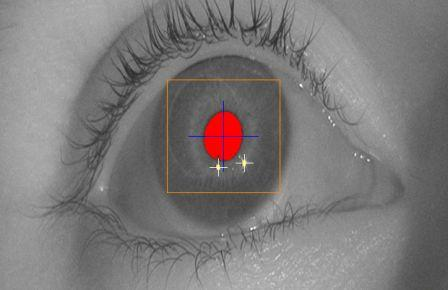
\includegraphics[width=0.5\textwidth, height=40mm]{figures/screenGazeTracker.jpg}
\vspace{-3mm}
\end{center}
\caption{\textbf{The Open Source ITU Gaze Tracker Tracking One Eye.} The
features tracked in the image are the pupil center and two corneal reflections. These features are used by the gaze 
estimation algorithms to determinine the PoR of the user on the screen.}
\label{screenGazeTracker}
\end{figure}

Depending on the hardware configuration of the different components, gaze tracking systems can be classified as either
\textit{remote} or \textit{head-mounted}. In remote systems, the camera and the light sources are detached from the
user, normally around the device screen, whereas in head-mounted systems the components are placed on the user's head, usually
mounted on a helmet or a pair of safety glasses \cite{lowcostitugazetracker}.

Head-mounted eye trackers can be used for mobile interaction as well as gaze estimation purposes.
In this work, we have build a low-cost headmounted eye tracker using off-the-shelf components.  The system consists of
safety glasses, batteries, wireless eye camera and the wireless scene or field of view camera. The wireless eye camera
and the associated software monitors the position of the pupil on the image and an infrared reflection in the iris. The
vector difference between the pupil center and the glint reflection in the iris can be tracked during a calibration
procedure to build a model of the user's gaze.

The calibration procedure consists on the user looking at a number of points on the environment and marking them on
the scene camera video stream while the user fixates on them.  Once a calibration procedure is completed, the gaze
estimation algorithm is able to determining the point of regard of the user in the environment.

We use the open-source Haytham \cite{Mardanbegi2011} software developed by Diako Mardanbegui at the IT University of
Copenhagen for mobile gaze estimation and extended it with a hand gesture recognition module that enables specific
interaction with objects in the environment through gaze and hand gestures.

Gesture recognition is a topic in computer science and language technology with the goal of interpreting human gestures
via mathematical algorithms. Gestures can originate from any bodily motion or state but commonly originate from the face
or hand.

An appealing feature of gestural interfaces is that they make possible for users to communicate with objects
without need for external control devices. Hand gestures are an obvious choice as a mechanism to interact with objects
in the environment. 

Automated hand gesture recognition is challenging since in order for such an approach to represent a serious alternative
to conventional input devices applications based on computer vision should be able to work successfully under
uncontrolled light conditions, no matter what kind of background the user stands in front of. In addition, deformable
and articulated objects like hands represent additional difficulty both for segmentation and shape recognition
purposes.

The hand gesture recognition module we develop here is able to detect a hand in front of the scene camera of the gaze
tracking glasses and it is also able to detect the number of fingers that the hand is holding up. We define the gesture
as holding the hand with a preset number of fingers hold up  for a predefined dwell time and moving it in a particular
direction: up, down, left  or right. The hand gesture recognition worked well for natural skin color, but using a latex glove of a
given color improves performance.

The system recognizes objects in the environment by detecting binary associated to them through the scene camera.

To interact with an object in the environment, the user of the glasses needs to first look at the binary beacon that
identifies the object and then performing the gesture. In this way, only that particular object in the environment 
will react to the hand gesture.


%---------------------------------------------------------------
\textbf{
\begin{center}
Method
\end{center}
}

Constructing the eye tracking glasses:

Materials:
Plastic safety glasses
Wireless camera with infra-red LEDs (eye camera)
Wireless camera	(scene camera)
Tin strips
Araldite
Steel wire
Tape
Double sided tape
9V battery
Tin snips

1. An area was traced onto the lens of the glasses where the eyes will be approximately when the user puts on the safety googles. 
2. Using the tin snips, the plastic part of the lenses bounded by the previously traced area was cut away. It is important that the
majority of the structure of the glasses is left intact to allow for stability.
3. Tin was cut to the size and shape of the infrared camera using the tin snips.
4. Steel wire was cut to a size of 25cm.
5. The steel wire was then attached to piece of tin using araldite.
6. Using double sided tape, the tin was attached to the back of the camera.
7. The steel wire was then bent into an 'L' shape and attached to the right side of the glasses (frame) using tape.
8. The wires for the battery were extended and the 9V battery was attached to the left side of the glasses to ensure that the glasses
are not unevenly balanced.
8. Using the haytham software, the position of the camera was checked to ensure the camera feed is filming the entire eye.
It was found that the best position of the eye is below the glasses so it doesn't obstruct the user's vision. 
8. The scene camera was mounted to the right of side of the glasses using sticky tape.



% ---------------------------------------------------------------
\noindent The method section of the extended summary should include information about participants, apparatus,
materials, procedure and analyses.
At a maximum you may use two full pages. Use the predefined format of this template and do not change the format in any
respect. For example, do not change the margins, font, font size, spacing between lines for either headers or text.
All sections (method, results and conclusion) need to be considered. But you are free to choose how much text you want
to include in each of these sections. If you are submitting a theoretical paper you may change the headers of the
sections method and results to something more appropriate.
If you need to include references in the extended summary they should follow APA standards and be included in full in
the text in square brackets, e.g., [Author, X. (2000). My amazing paper. \emph{Journal of Amazingology}, 3(21), pp.
1-2]. The extended summary is the basis for the reviewers. Notification of abstract acceptance for talks will be sent April 15
2013. We cannot guarantee that we will respect the authors' preferences for oral or poster presentation. Some talks may
be offered as poster presentations instead.



\textbf{Related Work}



%Related work on mobile gaze-based interaction, and hand gesture interaction with robot
\textbf{Combining gaze and gesture}
\textbf{Gaze for Interaction}
Point to demo video: \url{http://www.youtube.com/watch?v=tBOfvZboGfk}
%methods and limitations
\textbf{Gesture for Interaction}
%
\textbf{Gaze enhanced interaction }
%Pehaps different methods or modes that has been studied in our case
\texbf{Applications}
%Pehaps here we  can talk about different applications and then focued on our example in the next section



%---------------------------------------------------------------
\textbf{
\begin{center}
Experimental Example
\end{center}
}

For demonstration purposes, in the associated video \cite{gazetrackinglassesandhandgesturerecognitionVideo}, the system
presented here is used to interact with a computer, a breadboard with a set of light emitting diodes and with a robot


\textbf{}
%Hardware and softwares and the environment of our application

\textbf{}
%Different gestures, defining the method and steps

\begin{table}[\!ht]
	\centering
	\caption{This is a caption for the table}
	\vskip 0.12in
		\begin{tabular}{lcc}
			\hline
				& \multicolumn{2}{c}{Factor 2} \\
					\cline{2-3}
						Factor 1 & Condition A & Condition B \\
						\hline
						First  & 23(11) & 49(10) \\
						Second   & 22(12)  & 12(15) \\
						\hline
		\end{tabular}
	\label{ECEMtableTemplate}
\end{table}

For figures, use PNG, PSD, TIFF, BMP or JPG with a minimum resolution of 300 dpi. Figure 1 illustrates the style of a figure. The figure caption should be located below the figure.

\begin{figure}[h]
	\centering					\includegraphics[width=1.00\textwidth]{C:/ECEM.png}%Add file path and filenanme for your figure here
	\caption{This is a caption for the figure}
	\label{fig:ECEMfigureTemplate}
\end{figure}

%---------------------------------------------------------------
\textbf{
\begin{center}
Conclusion
\end{center}
}
%---------------------------------------------------------------
\noindent
In this work we have shown how to interact with objects in the environment through an innovative combination of
gaze and hand gestures. The method is easily extendable to multiple objects in the environment and a wide array of hand
gestures. The low-cost headmounted eye tracker does not compensate for parallax error, inability to differentiate
between the working plane and the calibration plane, and these can limit interaction with objects at a distance and
objects up close. We have tested the system  for interacting with a computer,  a breadboard and a mobile robot.
This work has demonstrated the feasibility of the approach as well as its usefulness.


\bibliographystyle{ieeetr}
\bibliography{library}



\end{document}